\documentclass[../main.tex]{subfiles}

\begin{document}
	\section{Installationsanleitung Allgemein}
	Durch den verwendeten Technologie-Stack lässt sich die Installation in kleinere Teilgebiete unterteilen. Die Voraussetzungen für eine erfolgreiche Installation sehen wie folgt aus:
	\begin{itemize}
		\item Java Version 11 oder höher
		\item Sofern der Spring-Boot-Server nicht als JAR-Datei vorhanden ist:
		\begin{itemize}
			\item Persönlicher GitHub-Account
			\item Gradle Version 7.3.+ oder Entwicklungsumgebung, die fähig ist, mit Gradle-Wrappern umzugehen.
		\end{itemize}
		\item Hosting-Angebot, das die Verwendung von Docker-Containern erlaubt
	\end{itemize}
	
	\subsection{Docker-Container}
	Der beabsichtigte Technologie-Stack sieht vor, dass zur erfolgreichen Inbetriebnahme zwei beziehungsweise drei Docker-Container verwendet werden.
	
	\subsubsection{Angular Frontend}
	\par Das Angular basierte Frontend wird durch den Spring Boot Server bereitgestellt. Bei der Erstellung des Servers wird dafür der Angular-Code kompiliert, optimiert und minimiert. Damit das Frontend auf die Korrekten Endpunkte zugreift, kann es nötig sein, die verwendeten Endpunkte anzupassen. Grundsätzlich reicht hierfür eine Anpassung vom \textit{basePath} in der Datei \texttt{environment.prod.ts} und eine weiter Anpassung vom \textit{API\_ENDPOINT} in der Datei \texttt{app-settings.ts}. Beide Dateien befinden sich im Unterordner \textit{paaq-client}.
	
	\subsubsection{Spring Boot Server}
	\par Durch die GitHub-Actions wird gewährleistet, dass auf DockerHub stets die aktuellste Version des Codes als Docker-Image verfügbar ist. Gemäss Grundeinstellungen der Actions ist dieses Image unter \textit{denadex/paaq} zu finden. 
	\par Die Anbindung an die Datenbank erfolgt über Parameter, die im Code gesetzt werden. Diese sind in der Datei \texttt{application.properties} im Unterordner \textit{paaq-server} aufgeführt.
	\par Zwischen dem Spring Boot Server und der Datenbank ist eine Verbindung essentiell. Das bedeutet, dass ein Port-Freigabe notwendig sein kann. Für genauere Angaben zum Setup einer Verbindung zwischen zwei Docker-Containern empfiehlt sich daher eine Konsultation des Hosting-Partners oder der Docker-Community.
	
	\subsubsection{MySQL Datenbank}
	\par Um über Docker-Container eine MySQL-Datenbank auszuführen, reicht es, das offizielle MySQL-Image zu verwenden. Dieses ist auf DockerHub unter \texttt{mysql} zu finden.
	\par Damit die anderen Container oder auch zusätzliche Dienste auf diese Datenbank zugreifen können, ist es notwendig, den Docker mit dem Parameter \texttt{MYSQL\_ROOT\_PASSWORD} zu starten. Als Passwort kann eine beliebige Zeichenfolge verwendet werden.
	\par Allfällige Daten aus früheren Datenbanken können mittels phpMyAdmin einfach in die neue MySQL-Datenbank eingepflegt werden.
	
	\subsubsection{phpMyAdmin}
	\par Ein phpMyAdmin-Container ist für den erfolgreichen Betrieb des Front- und Backends nicht notwendig. Wenn eine phpMyAdmin jedoch gewünscht ist, um tiefgründigere Einblicke in die Datenbank zu erhalten, kann ein solcher Container zusätzlich verwendet werden.
	\par Auch für phpMyAdmin gibt es ein offizielles Docker-Image. Um einen phpMyAdmin-Container mit dem Datenbankcontainer zu verknüpfen müssen die Parameter \texttt{PMA\_HOST} und \texttt{MYSQL\_ROOT\_PASSWORD} gesetzt werden.
	\par Analog zum Spring Boot Server muss auch hier gewährleistet werden, dass eine Verbindung zwischen den Containern tatsächlich existieren kann.
	
	\subsubsection{Container Networking}
	Der Spring Boot Server ist über Port 8080 erreichbar. Damit man die Webseite also von ausserhalb erreichen kann, müssen HTTP/S Requests an den Container auf Port 8080 weitergeleitet werden.
	
	\subsubsection{Externe Hilfestellungen}
	\begin{itemize}
		\item Informationen zum MySQL Docker Image: \href{https://hub.docker.com/_/mysql}{Offizielles MySQL Docker Image}
		\item Informationen zum phpMyAdmin Docker Image: \href{https://hub.docker.com/r/phpmyadmin/phpmyadmin/}{Offizielles phpMyAdmin Docker Image}
		\item Informationen zu Container Networking: \href{https://docs.docker.com/config/containers/container-networking/}{Docker Dokumentation}
	\end{itemize}
	
	%-------------------------------------------------------------------------------------------
	
	\subsection{Eigene Anpassungen}
	Folgend eine Kurzübersichtig über die nötigen Anpassungen, falls eine eigene individualisierte Lösung in Betracht gezogen wird.
	\subsubsection{Eigene GitHub-Fork}
	Das Projekt ist Open-Source und kann somit öffentlich eingesehen werden. Für eigene Änderungen kann das GitHub-Repository mittels 'forking' geklont werden. In der geklonten Fork kann man wie bei GitHub üblich seine eigenen Änderungen einpflegen.
	\subsubsection{Eigenes Docker Image}
	\par Für ein eigenes Docker-Image ist ein Benutzerkonto bei DockerHub notwendig. Anschliessend muss ein neues Repository bei DockerHub erzeugt werden. Damit der Code der eigenen GitHub-Fork auf dieses Docker-Repository gelangt, muss in den GitHub-Actions die neue URL für das DockerHub-Repository hinterlegt werden. Anzupassen sind:
	\begin{itemize}
		\item In \texttt{.github/workflows/build\_and\_publish.yml}: In der Rubrik 'Build and Publish' kann das Tag zu einem anderen Namen als 'paaq' abgeändert werden.
		\item In den Einstellungen des GitHub-Repositorys müssen zwei Secrets hinterlegt sein:
		\begin{itemize}
			\item \texttt{DOCKER\_HUB\_USERNAME}: Der Benutzername des DockerHub-Benutzerkontos.
			\item \texttt{DOCKER\_HUB\_ACCESS\_TOKEN}: Ein Access-Token für das DockerHub-Benutzerkontos.
		\end{itemize}
	\end{itemize}
	
	%-------------------------------------------------------------------------------------------
	
	\section{Installationsanleitung mit Sloppy.io}
	Da Sloppy.io das Erstellen und Verbinden von Containern, sowie auch die Verwendung einer neuen URL erheblich erleichtert, eignet es sich gut, um Prototypen zu Demonstrationszwecken zu hosten. Nachfolgend wird das Setup mittels Sloppy.io beschrieben.
	
	\subsection{Produktwahl}
	Für das Hosting der drei Docker-Container reicht der 'Basic' Plan der von Sloppy.io angebotenen Optionen aus. Sollte nach einiger Zeit der Speicher nicht mehr ausreichen oder mehr Rechenleistung nötig sein, können diese separat dazugekauft werden. Zusätzliche Features der Pläne 'Professional' und 'Business', wie beispielsweise 'External Logging' oder 'Custom Invoicing' sind für diesen Anwendungsfall unverhältnismässig. Ein Nachteil ist jedoch, dass Kollaboration mittels mehrerer Accounts erst mit dem teuersten Produkt möglich ist.
	
	\begin{figure}[H]
		\centering
		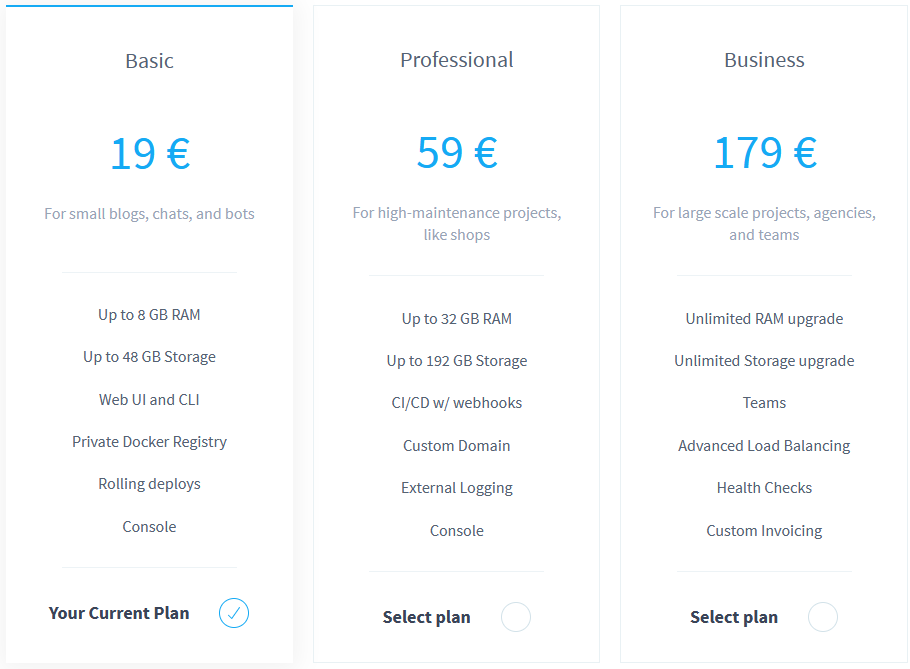
\includegraphics[width=0.8\textwidth]{../images/SloppyProductPlans} 
		\caption{Verschiedene Leistungsangebote von Sloppy.io}
		\label{fig:SloppyProductPlans}
	\end{figure}

	\subsection{Projekt erstellen}
	Sloppy.io ermöglicht es Benutzern, ihre Container bzw. Services in Projekten zu gliedern. Es ist daher zu empfehlen, für die drei Container ein eigenes Projekt anzulegen. Das Projekt sowie auch die Services können mit einem Namen versehen werden, der die Übersicht erleichtert. Pro Service können beliebig viele Container-Apps angegliedert werden. Es ist jedoch empfohlen, nur stark voneinander abhängige Container-Apps im selben Service laufen zu lassen.
	
	\begin{figure}[H]
		\centering
		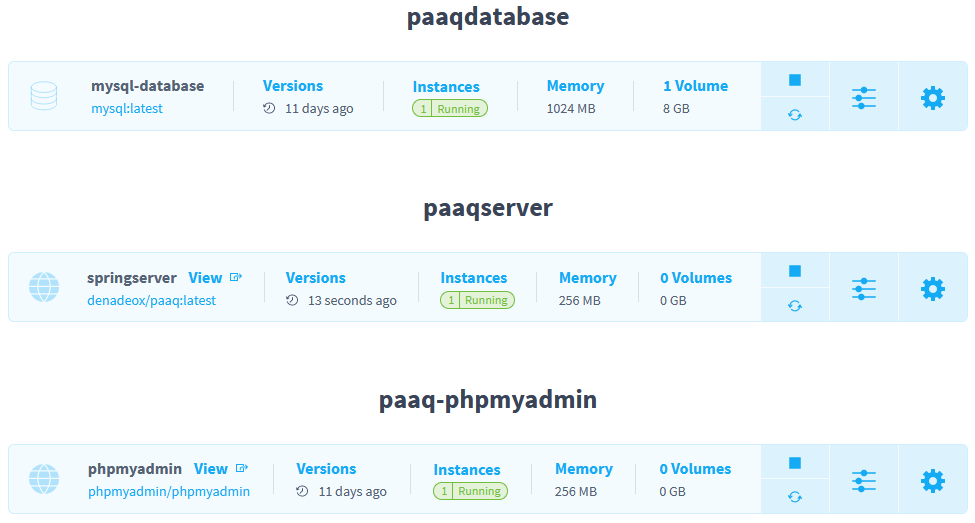
\includegraphics[width=0.8\textwidth]{../images/SloppyProjectStructure} 
		\caption{Strukturierung von Services und Apps in einem Sloppy-Projekt}
		\label{fig:SloppyProjectStructure}
	\end{figure}
	
	\subsection{MySQL-Datenbank}
	\par Für die Datenbank reicht es, per Sloppy.io ein neues App für einen entsprechenden Service anzulegen. Anschliessend kann das Docker-Image direkt per Name und optionalem Version-Tag verwendet werden. Folgende Umgebungsvariablen sind notwendig:
	\begin{itemize}
		\item \texttt{MYSQL\_ROOT\_PASSWORD}: Ein geeignetes Passwort für den Root-Nutzer der Datenbank.
	\end{itemize}
	\par Für einen effizienten Betrieb der Datenbank sollten der Container-App mindestens 512MB Arbeitsspeicher zugeschrieben werden. Im Verlaufe der Entwicklung hat sich ein 1024MB grosser Arbeitsspeicher bewährt.
	
	\subsection{phpMyAdmin}
	\par Ein phpMyAdmin-Container kann analog zum MySQL-Container an einen entsprechenden Service gekettet und per Sloppy.io-Dialog direkt von DockerHub verwendet werden. Da phpMyAdmin von extern zugänglich sein soll, wird die App als öffentlich eingestellt. Als URL kann eine eigene verwendet werden oder man nutzt eine kostenfreie Subdomain von Sloppy.io. 
	\par Folgende Umgebungsvariablen sind notwendig:
	\begin{itemize}
		\item \texttt{PMA\_HOST}: Sloppy ermöglicht es dem Benutzer hier direkt den MySQL-Container anzugeben.
		\item \texttt{MYSQL\_ROOT\_PASSWORD}: Ein geeignetes Passwort für den Root-Nutzer der Datenbank.
	\end{itemize}
	
	\begin{figure}[H]
		\centering
		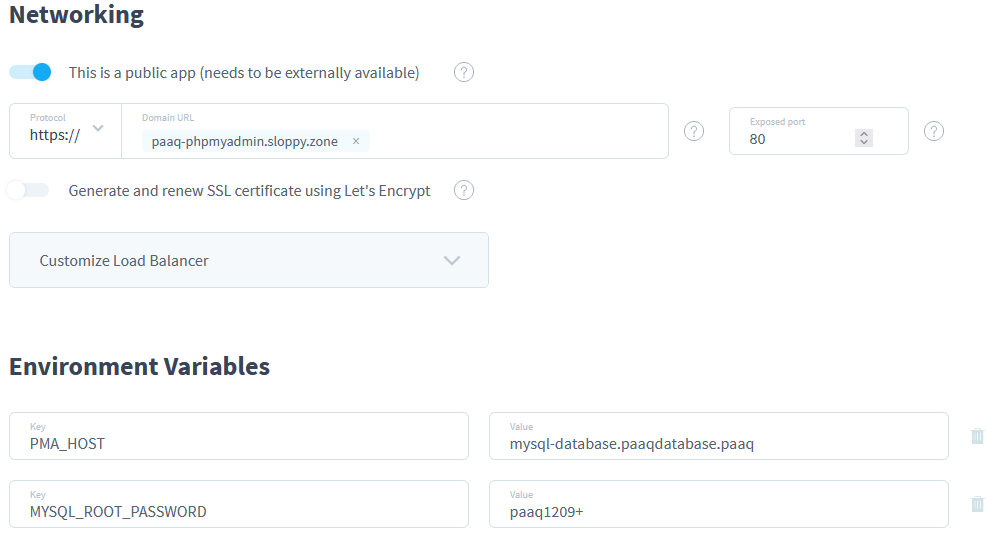
\includegraphics[width=0.8\textwidth]{../images/SloppyPHPPreferences} 
		\caption{Einstellungen für den phpMyAdmin Container.}
		\label{fig:SloppyPHPPreferences}
	\end{figure}
	
	\subsection{Spring Boot Server}
	\par Ein Docker-Container für den Spring Boot Server sollte ebenfalls in einem eigenen Service laufen. Analog zum phpMyAdmin- und dem MySQL-Container kann als Docker-Image dasjenige Image ausgewählt werden, dass auf DockerHub erstellt wurde. Der Spring Boot Server Container muss ebenfalls öffentlich sein und sollte auf den Port 8080 hören.
	\par Umgebungsvariablen sind keine nötig, da diese bereits im Container Image gesetzt sind.
	
	\begin{figure}[H]
		\centering
		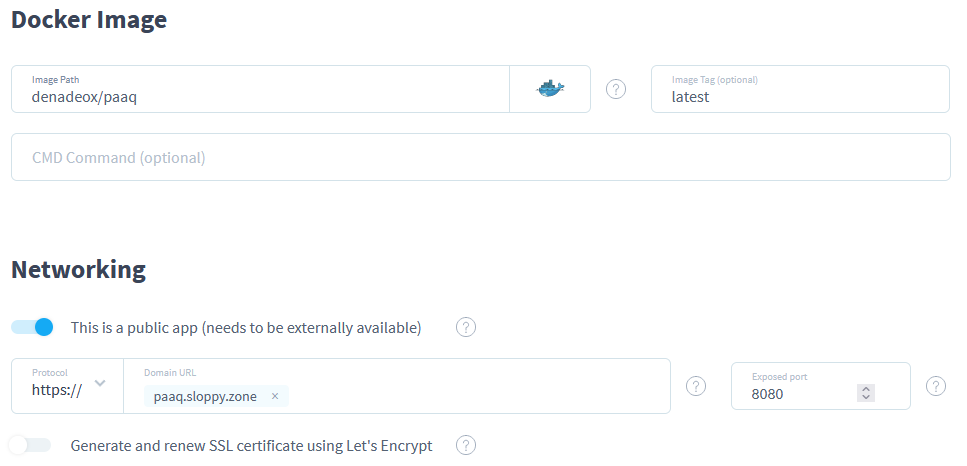
\includegraphics[width=0.95\textwidth]{../images/SloppySpringServer} 
		\caption{Der Spring Boot Server hört auf Port 8080.}
		\label{fig:SloppySpringServer}
	\end{figure}
	
	\subsection{Container Networking}
	\par Die einzelnen Container können über das interne Netzwerk von Sloppy.io iteinander kommunizieren. Die dazu notwendige interne URL eines Containers kann eingesehen werden und dementsprechend im Code für den Spring Boot Server zur Anbindung der Datenbank hinterlegt werden.
	\begin{figure}[H]
		\centering
		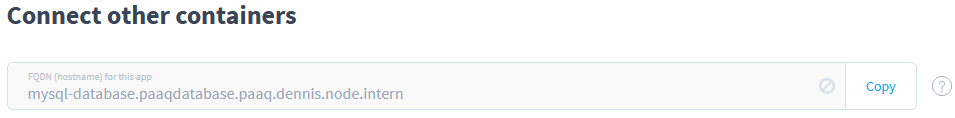
\includegraphics[width=0.95\textwidth]{../images/SloppyConnectContainers} 
		\caption{Sloppy.io Container haben eine Sloppy.io interne Adresse.}
		\label{fig:SloppyConnectContainers}
	\end{figure}
	
\end{document}